% **************************************************
% Macro specifiche per il documento corrente
% **************************************************
% Nome
\newcommand{\docName}{Piano di Progetto}
% Nome file
\newcommand{\docFileName}{piano\_di\_progetto.2.0.pdf}
% Versione
\newcommand{\docVers}{2.0}
% Data creazione
\newcommand{\creationDate}{2012-12-03}
% Data ultima modifica
\newcommand{\modificationDate}{2013-01-30}
% Stato in {Approvato, Non approvato}
\newcommand{\docState}{Approvato}
% Uso in {Interno, Esterno}
\newcommand{\docUsage}{Esterno}
% Destinatari da specificare come nome1\\ &nome2\\ ecc.
\newcommand{\docDistributionList}{Prof. Tullio Vardanega\\ & Prof. Riccardo Cardin}
% Redattori da specificare come nome1\\ &nome2\\ ecc.
\newcommand{\docAuthors}{Elena Zecchinato\\ &Andrea Meneghinello\\ &Stefano Farronato\\ &Marco Schivo \\ &Riccardo Tresoldi}
% Approvato da
\newcommand{\approvedBy}{Riccardo Tresoldi}
% Verificatori
\newcommand{\verifiedBy}{---}
% Perscorso (relativo o assoluto) che punta alla directory contenente shared/
% come sua sottodirectory (per comodità chiamiamola 'doc root').
\newcommand{\docRoot}{..}
% definire se si vuole l'indice delle tabelle
\def\INDICETABELLE{true}
% definire se si vuole l'indice delle figure
\def\INDICEFIGURE{true}

% importa il preambolo condiviso da tutti i documenti
% shared/preamble.tex
%
% Questo documento contiene la parte del preambolo condivisa e viene pertanto
% richiamato nel 'master' di tutti i documenti di progetto.  Al suo interno
% contiene le inclusioni (e le configurazioni) di tutti i package richiesti per
% la compilazione dei documenti, le macro di carattere generale e la definizione
% degli stili di pagina.

\documentclass[a4paper,10pt,openright]{article}

% **************************************************
% Macro generiche
% **************************************************
\newcommand{\team}{Software Synthesis}                    % chi siamo
\newcommand{\email}{software.synthesis@gmail.com}         % e-mail
\newcommand{\caName}{}                                    % titolo capitolato
\newcommand{\caDescr}{}                                   % descrizione
\newcommand{\inglese}[1]{\textit{#1}}

% **************************************************
% Codifica e lingua dei documenti
% **************************************************
\usepackage[utf8x]{inputenc}                              % codifica caratteri dei documenti sorgenti
\usepackage[english,italian]{babel}                       % localizzazione ai fini di sillabazione e cross-references
\usepackage[T1]{fontenc}                                  % codifica font di output

% **************************************************
% Definizione geometria della pagina
% **************************************************
\usepackage[a4paper,head=4cm,top=4.5cm,bottom=3cm,left=3cm,right=3cm,bindingoffset=5mm]{geometry}

% *************************************************
% Intestazioni e piè di pagina personalizzati
% *************************************************
\usepackage{fancyhdr}
% stile normale
\fancypagestyle{normal}{
\fancyhead{}                                              % intestazione
\fancyhead[RE,RO]{
\begin{picture}(0,0)
  \put(-410,0){
\includegraphics[width=1.02\textwidth]{header_logo}}
  \put(-410,10){\sffamily\large\leftmark}
\end{picture}
\vspace{-4pt}
}
\renewcommand{\headrulewidth}{.4pt}                       % riga sotto l'intestazione
\cfoot{}                                                  % piè di pagina
\fancyfoot[RO,LE]{\sffamily
  pag.~\thepage{} di \pageref{LastPage}}                  % a dx nelle pag. dispari e a sx in quelle pari
\fancyfoot[RE,LO]{\sffamily\docFileName{} -- v.\docVers}
\renewcommand{\footrulewidth}{.4pt}                       % riga sopra il piè di pagina
}
% stile per gli indici
\fancypagestyle{toc}{
\fancyhead{}                                              % intestazione
\fancyhead[RE,RO]{
\begin{picture}(0,0)
  \put(-410,0){
\includegraphics[width=1.02\textwidth]{header_logo}}
\end{picture}
}
\renewcommand{\headrule}{}                                % nessuna riga sotto l'intestazione
\cfoot{}                                                  % piè di pagina
\fancyfoot[RO,LE]{\sffamily\thepage{}}                    % a dx nelle pag. dispari e a sx in quelle pari
\fancyfoot[RE,LO]{\sffamily\docFileName{} -- v.\docVers}
\renewcommand{\footrulewidth}{.4pt}                       % riga sopra il piè di pagina
}

\pagestyle{fancy}                                         % premetto: non so usare bene le marche:
\renewcommand{\sectionmark}[1]{\markboth{#1}{#1}}         % se qualcuno ha idee migliori si faccia avanti!

% **************************************************
% Tabelle
% **************************************************
\usepackage{tabularx}                                     % tabelle di larghezza fissa con una o più colonne variabili
\usepackage{multirow}                                     % colonne con colonne che si estendono per più righe
\usepackage{booktabs}                                     % per inserire l'ambiente table e le righe orizz. nelle tabelle
\usepackage{longtable}			                          % tabelle oltre i limiti di pagina

% **************************************************
% Cross-references e collegamenti ipertestuali
% **************************************************
\usepackage[hidelinks]{hyperref}
\hypersetup{%
  colorlinks=false, linktocpage=false, pdfborder={0,0,0}, pdfstartpage=3, pdfstartview=FitV,%
  urlcolor=Cyan, linkcolor=Cyan, citecolor=Black, %pagecolor=Black,%
  pdftitle={\docName}, pdfauthor={\team}, pdfsubject={}, pdfkeywords={},%
  pdfcreator={pdflatex}, pdfproducer={pdflatex with hyperref package}%
}

% **************************************************
% Immagini e grafica
% **************************************************
\usepackage{graphicx}                                     % supporto ad aspetti avanzati delle immagini
\graphicspath{{\docRoot/pics/}}                           % percorso contenente tutti i file immagini
\usepackage{color}                                        % permette di colorare facilmente il testo

% **************************************************
% Altri pacchetti opzionali
% **************************************************     
\usepackage{lastpage}                                     % per sapere il numero totale di pagine
\usepackage{lipsum}                                       % genera "dummy text" per prove di impaginazione
\usepackage{eurosym}                                      % per il simbolo dell'euro usare \EUR{x} dove x è l'importo


\usepackage[italian]{varioref}

% Fine del preambolo e inizio del documento
\begin{document}

% Inclusione della prima pagina
% shared/firstpage.tex
%
% Questo documento definisce il contenuto della prima pagina, che si suppone
% essere uguale in tutti i documenti.  Oltre al logo e al titolo, la prima
% pagina contiene i metadati relativi al documento in cui viene inclusa.


% rimuove intestazioni e piè di pagina
\pagestyle{empty}

\begin{center}

% logo del gruppo

\includegraphics[width=1.5\textwidth]{logo}

\vspace{1in}

% titolo del documento
{\Huge\bfseries \docName}

\vspace{1in}

% tabella riepilogativa
\begin{tabularx}{.7\textwidth}{>{\bfseries\sffamily}l>{\sffamily}l}
\toprule
\multicolumn{2}{>{\sffamily}c}{Informazioni sul documento}\\
\midrule
Nome file:            & \docFileName\\
Versione:             & \docVers\\
Data creazione:       & \creationDate\\
Data ultima modifica: & \modificationDate\\
Stato:                & \docState\\
Uso:                  & \docUsage\\
Redattori:            & \docAuthors\\
Approvato da:         & \approvedBy\\
Verificatori:         & \verifiedBy\\
\bottomrule
\end{tabularx}

\end{center}

\newpage


% Storico delle modifiche
\section*{Storia delle modifiche}
\begin{longtable}{lp{.3\textwidth}lll}
\toprule
Versione & Descrizione intervento & Redattore & Ruolo & Data\\
\midrule % inserire qui il contenuto della tabella
2.4 & Aggiunta sezione del consuntivo relativa alla Progettazione di dettaglio e codifica& Andrea Rizzi & Responsabile & 2013-03-04\\
2.3 & Aggiornata sezione ``Analisi dei rischi'' alla data corrente & Andrea Rizzi & Responsabile & 2013-03-02\\
2.2 & Rimodellata sezione ``Pianificazione''& Andrea Rizzi & Responsabile & 2013-03-02\\
2.1 & Aggiunta sezione ``Vincoli'' e relative sottosezioni & Andrea Rizzi & Responsabile & 2013-03-02\\
2.0 & Approvazione documento & Riccardo Tresoldi & Responsabile & 2012-01-30\\
1.7 & Correzione errori lessico ortografici del documento riscontrati & Riccardo Tresoldi & Responsabile & 2012-01-29\\
1.6 & Inserimento diagramma Gantt di figura 10 e tabelle 17 e 18 relative alla sezione 7.1 & Riccardo Tresoldi & Responsabile & 2012-01-28\\
1.5 & Completa stesura sezione 7.1 & Riccardo Tresoldi & Responsabile & 2012-01-26\\
1.4 & Creazione e stesura preliminare del capitolo ``Consuntivo'' con la sezione relativa alla Progettazione Architetturale & Andrea Meneghinello & Responsabile & 2012-01-25\\
1.3 & Correzione ed integrazione della tabella 15 relativa al prospetto orario & Andrea Meneghinello & Responsabile & 2012-01-15\\
1.2 & Specifica dei documenti da consegnare in RP e RQ e modifica titolo relativo ala sezione ``Validazione'' & Andrea Meneghinello & Responsabile & 2012-01-15\\
1.1 & Correzione errori a livello ortografico e di terminologia riscontrati in fase di RR & Andrea Meneghinello & Responsabile & 2012-01-14\\
1.0 &Approvazione documento & Elena Zecchinato & Responsabile & 2012-12-20\\
0.14 &Verifica del documento & Diego Beraldin & Verificatore & 2012-12-20\\
0.13 &Inserimento tabelle nella sezione ``Preventivo'' & Marco Schivo & Amministratore & 2012-12-19\\
0.12 &Correzione contenuti nella ``Pianificazione'' & Stefano Farronato & Analista & 2012-12-18\\
0.11 &Inserimento Gantt, tabelle e immagini nella sezione ``Pianificazione'' & Marco Schivo & Amministratore & 2012-12-18\\
0.11 &Stesura e analisi sezione ``Validazione'' & Elena Zecchinato & Responsabile & 2012-12-18\\
0.10 &Stesura e analisi sezione `Progettazione di dettaglio e Codifica'' & Stefano Farronato & Responsabile & 2012-12-06\\
0.9 &Stesura e analisi sezione ``Progettazione Architetturale'' & Stefano Farronato & Responsabile & 2012-12-06\\
0.8 &Stesura e analisi sezione ``Analisi'', ``Ruoli e Costi'' & Andrea Meneghinello & Amministratore & 2012-12-05\\
0.7 &Stesura e analisi sezione ``Pianificazione'', ``Analisi'', ``Ruoli e Costi'' & Elena Zecchinato & Analista & 2012-12-05\\
0.6 &Stesura e analisi del ``Modello di ciclo di vita'' & Andrea Meneghinello & Amministratore & 2012-12-05\\
0.5 &Modifica sezione ``analisi dei rischi'' con introduzione e analisi di nuovi rischi, & Stefano Farronato & Responsabile & 2012-12-05\\
0.4 & Modifica sezione ``analisi dei rischi'' con introduzione e analisi di nuovi rischi, & Elena Zecchinato & analista & 2012-12-03\\
0.3 & Stesura ``Riferimenti'' & Stefano Farronato & Responsabile & 2012-12-03\\
0.2 & Stesura ``analisi dei rischi'' & Andrea Meneghinello & Amministratore & 2012-12-03\\
0.1 & Stesura scheletro documento, ``introduzione'' e introduzione preliminare dei ``rischi'' & Stefano Farronato & Responsabile & 2012-12-03\\
\bottomrule
\end{longtable}
\newpage

% inclusione dell'indice
% shared/toc.tex
%
% Questo file contiene le istruzioni che generano l'indice o gli indici del
% documento (utile nel caso in cui decidessimo di avere anche un indice delle
% tabelle e/o un indice delle figure).

\pagestyle{toc}
\pagenumbering{roman}

\tableofcontents

\newpage


% Alcuni aggiustamenti per le pagine
\pagenumbering{arabic}
\setcounter{page}{1}
\pagestyle{normal}

% Qui ha inizio il documento vero e proprio...
\section{Organigramma}
\begin{center}
\begin{tabularx}{0.8\textwidth}{c|c|c}
{\bf Nome}&{\bf Data}&{\bf Firma}\\ 
\hline
\multirow{2}{*}{Elena Zecchinato} &\multirow{2}{*}{ 2012-12-03} &\rule{3cm}{0cm} \\&&\\
\end{tabularx}
\end{center}

\subsection{Approvazione}
\begin{center}
\begin{tabularx}{0.8\textwidth}{c|c|c}
{\bf Nome}&{\bf Data}&{\bf Firma}\\ 
\hline
\multirow{2}{*}{Elena Zecchinato} & \multirow{2}{*}{2012-12-03} &\rule{3cm}{0cm} \\&&\\
\multirow{2}{*}{Tullio Vardanega} & \multirow{2}{*}{2013-01-09} &\rule{3cm}{0cm} \\&&\\
\end{tabularx}
\end{center}

\subsection{Accettazione componenti}
\begin{center}
\begin{tabularx}{0.9\textwidth}{c|c|c}
{\bf Nome}&{\bf Data}&{\bf Firma }\\ 
\hline
\multirow{2}{*}{Diego Beraldin} & \multirow{2}{*}{2012-12-03}&\rule{3cm}{0cm}\\&&\\
\multirow{2}{*}{Stefano Farronato} &\multirow{2}{*}{2012-12-03}&\\&&\\
\multirow{2}{*}{Andrea Meneghinello} &\multirow{2}{*}{2012-12-03}&\\&&\\
\multirow{2}{*}{Andrea Rizzi} &\multirow{2}{*}{2012-12-03}&\\&&\\
\multirow{2}{*}{Marco Schivo} &\multirow{2}{*}{2012-12-03}&\\&&\\
\multirow{2}{*}{Riccardo Tresoldi} &\multirow{2}{*}{2012-12-03}&\\&&\\
\multirow{2}{*}{Elena Zecchinato}&\multirow{2}{*}{2012-12-03}&\\&&\\
\end{tabularx}
\end{center}

\subsection{Componenti}
\begin{center}
\begin{tabularx}{0.9\textwidth}{c|c|l}
{\bf Nome}&{\bf Matricola}&{\bf e-mail}\\ 
\hline
\multirow{2}{*}{Diego Beraldin} & \multirow{2}{*}{1006523}&\multirow{2}{*}{diego.beraldin.1@studenti.unipd.it}\\&&\\
\multirow{2}{*}{Stefano Farronato} &\multirow{2}{*}{582726}&\multirow{2}{*}{stefano.farronato@studenti.unipd.it}\\&&\\
\multirow{2}{*}{Andrea Meneghinello} &\multirow{2}{*}{610762}&\multirow{2}{*}{andrea.meneghinello@studenti.unipd.it}\\&&\\
\multirow{2}{*}{Andrea Rizzi} &\multirow{2}{*}{610761}&\multirow{2}{*}{andrea.rizzi.9@studenti.unipd.it}\\&&\\
\multirow{2}{*}{Marco Schivo} &\multirow{2}{*}{619740}&\multirow{2}{*}{marco.schivo@studenti.unipd.it}\\&&\\
\multirow{2}{*}{Riccardo Tresoldi} &\multirow{2}{*}{610068}&\multirow{2}{*}{riccardo.tresoldi@studenti.unipd.it}\\&&\\
\multirow{2}{*}{Elena Zecchinato}&\multirow{2}{*}{1007584}&\multirow{2}{*}{elena.zecchinato.1@studenti.unipd.it}\\&&\\
\end{tabularx}
\end{center}

\clearpage
\section{Introduzione}
\subsection{Scopo del prodotto}
\purpose

\subsection{Scopo del documento}
Il seguente documento ha lo scopo di presentare e definire i ruoli professionali dei membri del team di lavoro dell'azienda Software Synthesis sul progetto ``\caName'' regolarmente accettato dall'azienda appaltatrice Zucchetti s.r.l

Sono inoltre descritti i costi stimati necessari al completamento di tale progetto e i rischi possibili nella sua realizzazione. Infine viene stilato il carico di lavoro distribuito per ogni soggetto del team mediante un organigramma specificante tempo e risorse.

\subsection{Glossario}
\glossaryIntro

\section{Riferimenti}

\subsection{Normativi}
\begin{itemize}
\item[] \textit{Vincoli di organigramma}: Specificati dal Committente designato all'indirizzo\\ \url{http://www.math.unipd.it/~tullio/IS-1/2012/Progetto/PD01b.html};
\item[] \textit{norme\_di\_progetto.3.0.pdf} allegato;
\end{itemize}

\subsection{Informativi}
\begin{itemize}
\item[] Capitolato d'appalto: MyTalk, v1.0, redatto e rilasciato dal proponente Zucchetti s.r.l reperibile all'indirizzo: \\ \url{http://www.math.unipd.it/~tullio/IS-1/2012/Progetto/C1.pdf};
\item[] Testo di consultazione: \textit{Software Engineering (8th edition) Ian Sommerville, Pearson Education | Addison-Wesley}.
\end{itemize}
\clearpage

\section{Modello di ciclo di vita}
Per lo sviluppo del prodotto MyTalk, il team di Software Synthesis ha optato per il modello di ciclo di vita incrementale.

L'inesperienza dei membri del gruppo porta infatti ad escludere il ciclo di vita sequenziale, che pur essendo il modello che si adatta maggiormente alla conformazione sequenziale delle scadenze, richiede una certa esperienza a causa della sua rigidità che non prevede la possibilità di ritornare nelle varie attività del progetto, una volta che sono state abbandonate.

Il modello di ciclo di vita evolutivo è stato altresì scartato in quanto ritenuto oneroso sia dal punto di vista economico che temporale visto che richiede un continuo attraversamento delle attività del ciclo di vita, che potrebbe portare, data l'inesperienza del gruppo, ad una convergenza molto lenta e quindi discostarsi anche di molto dalla pianificazione di tempi e costi.

Il ciclo di vita scelto dal team è quindi quello incrementale, che permette la realizzazione del prodotto per passi pianificati,in modo da poter gestire l'intero svolgimento progettuale nei tempi e nei costi previsti.

Questo tipo di modello inoltre permetterà di sviluppare e completare il software sviluppando i requisiti minimi obbligatori imposti dal committente generando quindi un programma prototipale nel quale sarà possibile presentare al proponente un prodotto funzionante comprensivo delle funzionalità essenziali. Il software verrà in seguito completato procedendo all'integrazione dei requisiti facoltativi e desiderabili presi in considerazione rendendo definitivo lo sviluppo del prodotto.

Concludiamo quindi specificando che il modello sarà composto da due incrementi.

Basandoci sulle specifiche dettate da questo tipo di modello, il team svolgerà inizialmente (e una sola volta) le attività di analisi e progettazione a livello architetturale ad alto livello, successivamente si lavorerà iterativamente sul controllo e la valutazione della realizzazione nel dettaglio.


\section{Vincoli}
\subsection{Ruoli e Costi}
I ruoli costituiscono delle funzioni aziendali che vengono assegnate al progetto. La tabella 1 riporta i ruoli che devono essere ricoperti da tutti i membri del team e i rispettivi costi orari:

\begin{table}[h]
\centering
\begin{tabular}{|l|c|}
\hline
Ruolo& Costo Orario\\
\hline
Responsabile & \EUR{30}\\
Amministratore  & \EUR{20}\\
Analista & \EUR{25}\\
Progettista  & \EUR{22}\\
Programmatore & \EUR{15}\\
Verificatore & \EUR{15}\\
\hline
\end{tabular}
\caption{costo orario per ruolo}
\end{table}

\subsection{Rotazione ruoli}
Al fine di permettere che ogni membro del gruppo possa ricoprire almeno una volta ogni ruolo, per trarre il massimo beneficio da tale esperienza è stato imposto un meccanismo di rotazione delle attività.

Tale meccanismo dovrà garantire, oltre alla già citata rotazione, che non vi siano conflitti di interesse, ovvero ad esempio non ci siano periodi in cui una stessa risorsa sia verificatrice di se stessa.

Qualora siano necessarie delle modifiche in seguito alla consegna di un documento, coloro che svolgeranno il ruolo di verificatore potrebbero figurare fra i redattori dello stesso in una fase temporale precedente. Si tratta di un evento inevitabile pertanto si eviteranno i conflitti facendo sì che i verificatori controllino solo le parti che non erano state redatte da loro.

\subsection{Vincoli economici e temporali}
Il progetto ha un vincolo economico definito e non sarà accettata nessuna proposta con una pianificazione inferiore a \EUR{13.000} totali; inoltre è prefissata una soglia minima di impegno orario per singolo soggetto di 85 ore produttive, l'impegno massimo è invece imposto a 105 ore personali per lo sviluppo dell'intero progetto.

\subsection{Scadenze temporali}
Al fine di consentire una valutazione sullo stato di avanzamento dello sviluppo del progetto che il team Software Synthesis ha preso in consegna, il gruppo ha deciso di rispettare le seguenti scadenze sulle quali si baserà la pianificazione del progetto:
\begin{itemize}
\item Revisione Requisiti (RR): 2012-01-10
\item Revisione di Progetto (RP): 2013-02-05
\item Revisione di Qualifica (RQ): 2013-03-07
\item Revisione di Accettazione (RA): indicativamente ipotizzata al 2013-03-25
\end{itemize}
Il gruppo si impegna ad esporre in Revisione di Progetto la progettazione architetturale (PA) ad alto livello del prodotto finale.
\clearpage

\section{Pianificazione}
Per consentire una corretta gestione delle scadenze esposte nella sezione precedente, il team ha deciso di impostare lo sviluppo del progetto in quattro attività:

\begin{itemize}
\item Analisi dei Requisiti
\item Progettazione Architetturale
\item Progettazione di Dettaglio e Codifica
\item Validazione 
\end{itemize}

Di seguito verranno analizzate dettagliatamente le attività citate.

\subsection{Analisi dei Requisiti}
Questa attività inizia in data 2012-11-29 e finisce in data 2013-01-10. Tuttavia la data di consegna dei documenti che descrivono le attività di analisi dei requisiti è prevista il giorno 2012-12-21, restringendo il tempo produttivo effettivo.

Questa attività coinvolge i ruoli di Responsabile, Amministratore, Analista e Verificatore. Le ore svolte dai vari componenti in questa attività non rientrano nel preventivo, l'attività di analisi dei requisiti costituisce infatti un investimento da parte dell'azienda e non può quindi essere a carico del proponente ne faranno parte del massimo complessivo finale di 100 ore lavorative per componente .

Verrà in ogni caso tenuto traccia del dettaglio delle ore compiute per la già concordata rotazione dei ruoli dei membri del team. A tale proposito già in questa attività preliminare sono state concordate due fasi (la prima terminerà il 2012-12-10), in modo da permettere lo scambio degli incarichi tra i soggetti.

Durante questo periodo verrà svolto principalmente un lavoro di studio a livello di fattibilità del progetto e un'attenta analisi dei requisiti. 

\begin{figure}[h!]
  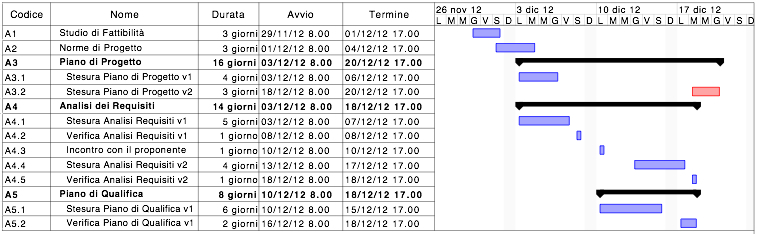
\includegraphics[width=\textwidth]{Analisi}
\caption{Gantt della pianificazione dell'attività di Analisi dei Requisiti}
\end{figure}
\clearpage
In questa attività i ruoli sono definiti come in tabella \ref{tab:ruolian}.
\begin{table}[h!]
\centering
\begin{tabular}{|l|c|c|c|c|c|c|}
\hline
Componente& RE& AM& AN& PRO& PRG& VER\\
\hline
Diego Beraldin & & & 10& & & 10\\
Stefano Farronato & 8& & 13& & & \\
Andrea Meneghinello & & 6& 15& & & \\
Andrea Rizzi & & & 21& & & \\
Marco Schivo & & 12& & & & 10\\
Riccardo Tresoldi & & & 21& & & \\
Elena Zecchinato & 8& & 12& & & \\
\hline
Totale & 16& 18& 82& & & 20\\
\hline
\end{tabular}
\caption{copertura ruoli nell'attività di Analisi dei Requisiti}\label{tab:ruolian}
\end{table}

Ad ogni risorsa sarà distribuito il seguente carico di lavoro (figura \ref{fig:ruolian}):

\begin{figure}[h!]
\centering
  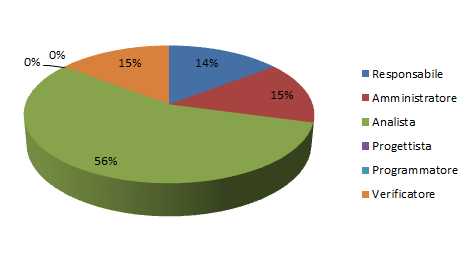
\includegraphics{torta_analisi}
\caption{Torta ripartizione ruoli nell'attività di Analisi dei Requisiti}\label{fig:ruolian}
\end{figure}
\clearpage

Infine vengono fornite le ore distinte per componente del team che sono state svolte in questa attività (tabella \ref{tab:ruolian2}) e la copertura dei ruoli sempre divisa per soggetto (tabella \ref{tab:ruolian3}):

\begin{table}[h!]
\centering
\begin{tabular}{|l|c|c|c|}
\hline
Componente& Fase I& Fase II& Totale\\
\hline
Diego Beraldin &10 &10 & 20\\
Stefano Farronato & 8& 13& 20\\
Andrea Meneghinello & 6& 15& 21\\
Andrea Rizzi & 11& 10& 21\\
Marco Schivo & 10& 12& 22\\
Riccardo Tresoldi & 10& 11& 21\\
Elena Zecchinato & 12& 8& 20\\
\hline
\end{tabular}
\caption{copertura ruoli nell'attività di Analisi dei Requisiti}\label{tab:ruolian2}
\end{table}

\begin{table}[h!]
\centering
\begin{tabular}{|l|c|c|}
\hline
Componente& Fase I&Fase II\\
\hline
Diego Beraldin & analista&verificatore\\
Stefano Farronato & responsabile&analista\\
Andrea Meneghinello & amministratore&analista\\
Andrea Rizzi &  analista&analista\\
Marco Schivo & verificatore&amministratore\\
Riccardo Tresoldi & analista&analista\\
Elena Zecchinato & analista&responsabile\\
\hline
\end{tabular}
\caption{ruoli per persona nell'attività di Analisi dei Requisiti}\label{tab:ruolian3}
\end{table}

Come si evince dalle ore di lavoro assegnate ai verificatori, nel corso dello svolgimento dell'attività di analisi dei requisiti sono stati effettuati controlli di verifica sui singoli documenti prodotti al fine di assicurarne la conformità con le norme.
\clearpage

\subsection{Progettazione Architetturale}
Questa attività inizia in data 2013-01-09 e finisce in data 2013-01-31, per un totale di 20 giorni lavorativi. Allo scadere di tale termine il team intende aggiungere alla lista dei documenti già presentati a seguito dell'attività di analisi dei requisiti il documento relativo alla specifica tecnica denominato \textit{specifica\_tecnica.1.0.pdf}.

Questa attività coinvolge i ruoli di Responsabile, Amministratore, Analista, Progettista e Verificatore.
L'analista in questo periodo temporale avrà un ruolo prevalentemente rifinitorio (ma doveroso) nei confronti dell'analisi dei requisiti, 

Durante questa attività è stato pianificato un ulteriore lavoro rifinitorio di analisi, in modo da produrre un documento finale che descriva in modo chiaro e completo i requisiti necessari a rendere il prodotto conforme a quanto richiesto e per rendere più sicuro e corretto possibile l'avvio progettuale della Specifica Tecnica.
La fase di progettazione ad alto livello che si andrà quindi a stilare descriverà le funzionalità principali atte a soddisfare i requisiti emersi nell'analisi.

Si è deciso di suddividere questo periodo in due fasi. La prima fase termina il 2013-01-21 e ed inizia la seconda, il seguente diagramma di Gantt descrive la pianificazione dei compiti:

\begin{figure}[h]
  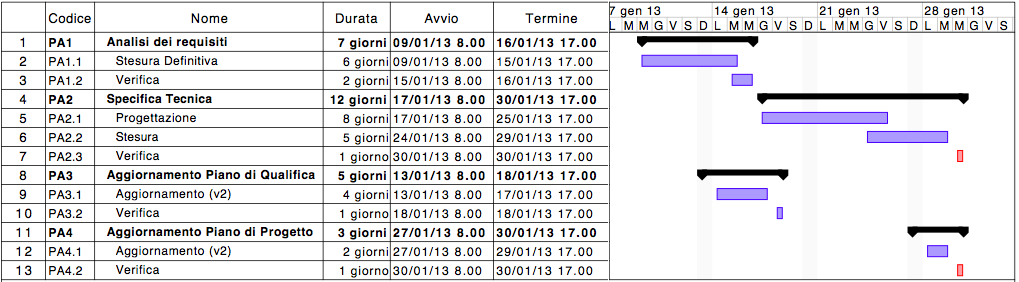
\includegraphics[width=\textwidth]{Progettazione_Architetturale}
\caption{Gantt della Progettazione Architetturale}\label{fig:ganttprog}
\end{figure}

In questa attività i ruoli sono definiti come in tabella \ref{tab:ruoliprog}:

\begin{table}[h]
\centering
\begin{tabular}{|l|c|c|c|c|c|c|c|c|}
\hline
\multirow{2}{*}{Componente}& RE& AM& AN& PRO& PRO& PRG& VER& VER\\
                    &    &      &      &fase1          &fase2         &        &fase1	 &fase2\\ 
\hline
Diego Beraldin & & 5& 13& & 17& & &\\
Stefano Farronato & & & & 22& & & & 16\\
Andrea Meneghinello & 9& & & 12& & & & 13\\
Andrea Rizzi & & 8& & & 16& & 16& \\
Marco Schivo & & & 15& & 20& & & \\
Riccardo Tresoldi & 7& & & 18& & & & 11\\
Elena Zecchinato & & & & & 10& & 25& \\
\hline
Totale & 16& 13& 28& 52& 63& & 41& 40\\
\hline
\end{tabular}
\caption{copertura ruoli nell'attività di Progettazione Architetturale}\label{tab:ruoliprog}
\end{table}
\clearpage

Ad ogni risorsa sarà distribuito il seguente carico di lavoro (figura \ref{fig:ruoliprog}):
\begin{figure}[h!]
\centering
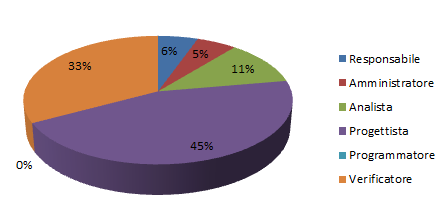
\includegraphics{torta_PA}
\caption{Torta ripartizione ruoli nell'attività di Progettazione Architetturale}\label{fig:ruoliprog}
\end{figure}

Infine vengono fornite le ore distinte per componente del team che sono state svolte in questa attività (Tabella \ref{tab:ruoliprog2}) e la copertura dei ruoli sempre divisa per soggetto (tabella \ref{tab:ruoliprog3}):

\begin{table}[h!]
\centering
\begin{tabular}{|l|c|c|c|}
\hline
Componente& Fase I& Fase II& Totale\\
\hline
Diego Beraldin &18 &17 & 35\\
Stefano Farronato & 22& 16& 38\\
Andrea Meneghinello & 21& 13& 34\\
Andrea Rizzi & 16& 24& 40\\
Marco Schivo & 15& 20& 35\\
Riccardo Tresoldi & 18& 18& 36\\
Elena Zecchinato & 25& 10& 35\\
\hline
\end{tabular}
\caption{copertura ruoli nell'attività di progettazione architetturale}\label{tab:ruoliprog2}
\end{table}

\begin{table}[h!]
\centering
\begin{tabular}{|l|c|c|}
\hline
Componente& Fase I&Fase II\\
\hline
Diego Beraldin & amministratore/analista&progettista\\
Stefano Farronato & progettista&verificatore\\
Andrea Meneghinello & responsabile/progettista&verificatore\\
Andrea Rizzi &  verificatore&amministratore/progettista\\
Marco Schivo & analista&progettista\\
Riccardo Tresoldi & progettista&responsabile/verificatore\\
Elena Zecchinato & verificatore&progettista\\
\hline
\end{tabular}
\caption{ruoli per persona nell'attività di progettazione architetturale}\label{tab:ruoliprog3}
\end{table}

Il risultato della progettazione architetturale è stato inoltre sottoposto a un'accurata attività di verifica, com'è possibile inferire dal numero di ore che sono state assegnate ai verificatori durante il periodo di tempo in esame.
\clearpage

\subsection{Progettazione di Dettaglio e Codifica}
La seguente attività inizia in data 2013-02-07 e terminerà in data 2013-03-06. In questo periodo si svilupperà la progettazione di dettaglio del prodotto MyTalk e la sua codifica. Verranno presentati i documenti \textit{definizione\_di\_prodotto.1.0.pdf} e \textit{manuale\_utente.1.0.pdf}.

In questa periodo temporale, coerentemente con il modello di ciclo di vita scelto, l'attività di Progettazione di Dettaglio e la Codifica avverranno per \underline{iterazioni}.
Sono previste 2 iterazioni, nella prima si procederà con la progettazione di dettaglio, nonchè l'inizio dell'attività di codifica sulle funzionalità principali che il prodotto dovrà possedere.
Al termine di questa prima iterazione si avrà a disposizione un primo \underline{prototipo} per testare le funzioni principali dell'applicativo MyTalk, in data 2013-02-22.
È stata scelta tale data anche per provvedere ad una doverosa rotazione di ruoli all'interno del team di sviluppo, per consentire a tutti i soggetti di raggiungere il massimo apprendimento pratico dei vari compiti.
Nella seconda iterazione si andranno ad integrare le funzionalità avanzate al prodotto e valutato cosa sia migliorabile ed eventualmente aggiunto a quanto realizzato.

Al fine di ridurre (auspicabilmente) al minimo le difficoltà di programmazione sono state dedicate una quantità rilevante di ore all'attività di progettazione, e al fine di evitare conflitti di interesse dovuti alle già citate ``autocorrezioni'' i membri del team potranno verificare soltanto moduli implementati da terzi. Analogamente i progettisti che nella seconda iterazione avranno un ruolo di programmatore scriveranno codice che implementa la progettazione di un altro componente del gruppo.

Il diagramma di Gantt in figura \ref{fig:gantdc} descrive l'organizzazione lavorativa:

\begin{figure}[h!]
  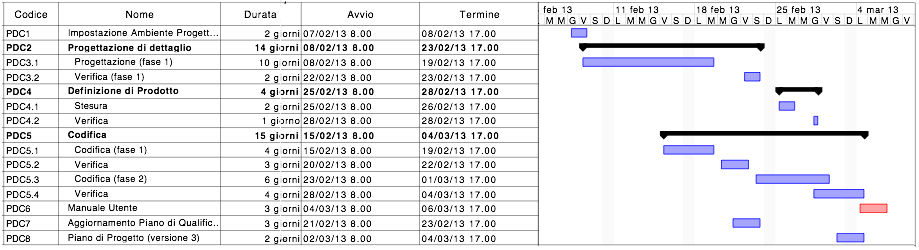
\includegraphics[width=\textwidth]{Progettazione_di_Dettaglio_e_Codifica}
\caption{Gantt della Progettazione di Dettaglio e Codifica}\label{fig:gantdc}
\end{figure}

In questa attività i ruoli sono definiti come in tabella \ref{tab:ruolidc}:

\begin{table}[h!]
\centering
\begin{tabular}{|l|c|c|c|c|c|c|c|c|}
\hline
\multirow{2}{*}{Componente}& RE& AM& AN& PRO& PRG&VER& PRG& VER \\
					      &    &     &      &        & fase1&fase1&fase2&fase2\\
\hline
Diego Beraldin & 9& & & & 24& & & 15\\
Stefano Farronato & & 5& & 10&14 & & & 18\\
Andrea Meneghinello & & & & & & 25& 19& \\
Andrea Rizzi & 9& & & 22& & & 12& \\
Marco Schivo & & & & 16& 10& & & 20\\
Riccardo Tresoldi & & 7& & & & 20& 20& \\
Elena Zecchinato & & & & 25& & & 20& \\
\hline
Totale & 18& 12& 0& 73& 48& 45& 71& 53\\
\hline
\end{tabular}
\caption{copertura ruoli nell'attività di Progettazione di Dettaglio e Codifica}\label{tab:ruolidc}
\end{table}
\clearpage

Ad ogni risorsa sarà distribuito il seguente carico di lavoro (figura \ref{fig:ruolidc}):

\begin{figure}[h!]
\centering
  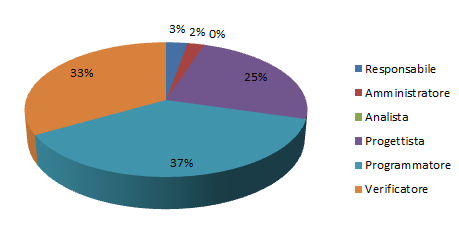
\includegraphics{torta_PDC}
\caption{Torta ripartizione ruoli nell'attività di Progettazione di Dettaglio e Codifica}\label{fig:ruolidc}
\end{figure}

Infine vengono fornite le ore distinte per componente del team che sono state svolte in questa attività (tabella \ref{tab:ruolidc2})e la copertura dei ruoli sempre divisa per soggetto (tabella \ref{tab:ruolidc3}):

\begin{table}[h]
\centering
\begin{tabular}{|l|c|c|c|}
\hline
Componente& Fase I& Fase II& Totale\\
\hline
Diego Beraldin & 31& 15& 48\\
Stefano Farronato & 29& 18& 47\\
Andrea Meneghinello & 25& 19& 44\\
Andrea Rizzi &22 &21 & 43\\
Marco Schivo & 26& 20& 46\\
Riccardo Tresoldi & 27& 20& 47\\
Elena Zecchinato & 25& 20& 45\\
\hline
\end{tabular}
\caption{copertura ruoli nell'attività di progettazione di dettaglio e codifica}\label{tab:ruolidc2}
\end{table}

\begin{table}[h!]
\centering
\begin{tabular}{|l|c|c|}
\hline
Componente& Fase I&Fase II\\
\hline
Diego Beraldin & responsabile/programmatore&verificatore\\
Stefano Farronato & progettista/programmatore&amministratore/verificatore\\
Andrea Meneghinello & verificatore&programmatore\\
Andrea Rizzi &  progettista&responsabile/verificatore\\
Marco Schivo & progettista/programmatore&verificatore\\
Riccardo Tresoldi & amministratore/verificatore&programmatore\\
Elena Zecchinato & progettista&programmatore\\
\hline
\end{tabular}
\caption{ruoli per persona nell'attività di dettaglio e codifica}\label{tab:ruolidc3}
\end{table}

Il risultato delle attività di progettazione di dettaglio e codifica è inoltre sottoposto a verifica prima della conclusione.

\clearpage

\subsection{Validazione}

Questa attività inizia in data 2013-03-05 e finisce in data 2013-03-22, per un totale di 16 giorni \underline{lavorativi}. In tale data verrà consegnata la versione definitiva di tutta la documentazione. Coinvolge i ruoli di Responsabile, Amministratore, Progettista, Programmatore e Verificatore. Si può notare che non è più attivo quindi il ruolo di Analista, si prevede infatti che a questo stadio del progetto l'attività di analisi sia ovviamente conclusa.

L'attività di validazione è da intendersi come un controllo a posteriori sul prodotto finale al fine di verificarne l'aderenza ai requisiti di sistema e utente ed effettuarne il collaudo definitivo, l'attività di verifica è stata invece svolta durante l'intero processo di sviluppo, come evidenziato in precedenza, di volta in volta al termine di ognuna delle attività precedentemente elencate.

Si è deciso di inserire  in questo periodo anche il ruolo del programmatore in quanto si prevede che qualche ora di codifica potrebbe risultare necessaria al fine di terminare lo sviluppo del software iniziato nelle attività precedenti.

Non si è ritenuta necessaria la suddivisione in fasi del periodo visto che le attività riguardano in gran parte il \underline{processo} di validazione e quindi non vi è necessità di una forte rotazione.

Essendoci però la presenza dei ruoli di progettista e programmatore per un numero limitato di ore e la necessità di impiegare risorse nel ruolo di verificatore, sarà necessario impiegare le persone che svolgono tali ruoli nelle attività di validazione.  

Nell'assegnazione dei ruoli si è volta particolare attenzione al conflitto di interessi,  progettando una distribuzione tale da evitare la situazione surreale in cui un verificatore controlli il suo stesso operato.

Il diagramma di Gantt in figura \ref{fig:gantvv} descrive l'organizzazione lavorativa:

\begin{figure}[h!]
  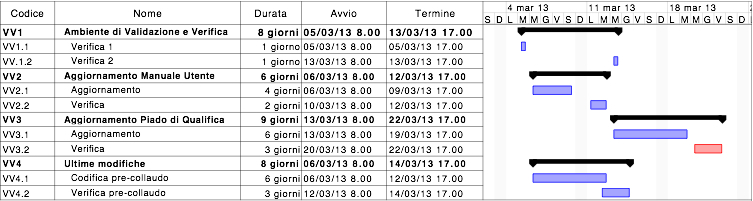
\includegraphics[width=\textwidth]{Verifica_e_Validazione}
\caption{Gantt della Validazione}\label{fig:gantvv}
\end{figure}

In questa attività i ruoli sono definiti come in tabella \ref{tab:ruolivv}:

\begin{table}[h!]
\centering
\begin{tabular}{|l|c|c|c|c|c|c|}
\hline
Componente& RE& AM& AN& PRO& PRG& VER\\
\hline
Diego Beraldin & & & & & & 20\\
Stefano Farronato & & & & & 5& 18\\
Andrea Meneghinello & & & & 5& & 15\\
Andrea Rizzi & & & & & & 20\\
Marco Schivo & 6& & & & & 16\\
Riccardo Tresoldi & & & & & & 20\\
Elena Zecchinato & & 8& & & & 15\\
\hline
Totale & 6& 8& 0& 5& 5& 124\\
\hline
\end{tabular}
\caption{copertura ruoli nell'attività di Validazione}\label{tab:ruolivv}
\end{table}
\clearpage

Ad ogni risorsa sarà distribuito il seguente carico di lavoro (figura \ref{fig:ruolivv}):

\begin{figure}[h!]
\centering
  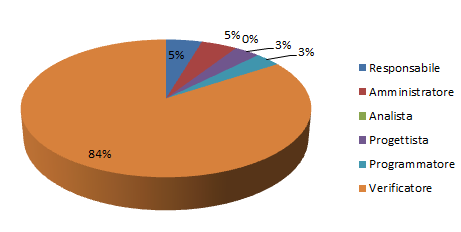
\includegraphics{torta_VV}
\caption{Torta ripartizione ruoli nell'attività di Validazione}\label{fig:ruolivv}
\end{figure}

Infine vengono fornite le ore distinte per componente del team che sono state svolte in questa attività (tabella \ref{tab:ruolivv2})e la copertura dei ruoli sempre divisa per soggetto (tabella \ref{tab:ruolivv3}):

\begin{table}[h]
\centering
\begin{tabular}{|l|c|}
\hline
Componente& Totale \\
\hline
Diego Beraldin & 20\\
Stefano Farronato & 23\\
Andrea Meneghinello & 20\\
Andrea Rizzi & 20\\
Marco Schivo & 22\\
Riccardo Tresoldi & 20\\
Elena Zecchinato & 23\\
\hline
\end{tabular}
\caption{copertura ruoli nell'attività di Validazione}\label{tab:ruolivv2}
\end{table}

\begin{table}[h!]
\centering
\begin{tabular}{|l|c|c|}
\hline
Componente& Attività\\
\hline
Diego Beraldin &verificatore\\
Stefano Farronato & programmatore/verificatore\\
Andrea Meneghinello &progettista/verificatore\\
Andrea Rizzi &verificatore\\
Marco Schivo &responsabile/verificatore\\
Riccardo Tresoldi &verificatore\\
Elena Zecchinato &amministratore/verificatore\\
\hline
\end{tabular}
\caption{ruoli per persona nell'attività di Validazione}\label{tab:ruolivv3}
\end{table}
\clearpage

\section{Preventivo}

\subsubsection{Prospetto Orario}
La tabella \ref{tab:oretotali} illustra le ore totali di lavoro \underline{produttivo} di ciascun membro del team Software Synthesis, per soggetto è stato preventivato un totale di 103 ore produttive, pertanto coerenti con le richieste vincolanti.\footnote{%
  Le celle contrassegnate da una `A' rappresentano le ore di lavoro impiegate durante lo svolgimento dell'analisi dei requisiti, che non contribuiscono al monte ore totale di ciascuno dei componenti del gruppo.
}

\begin{table}[h]
\centering
\begin{tabular}{|l|c|c|c|c|c|c|c|}
\hline
Componente& RE& AM& AN& PRO& PRG& VER& TOTALE\\
\hline
Diego Beraldin & 9& 5& 13& 17& 24& 35& 103\\
Stefano Farronato & A& 5& A& 32& 14& 52&  103\\
Andrea Meneghinello & 9& A& A& 17& 24& 53& 103\\
Andrea Rizzi & 9& 8& A& 38& 12& 36& 103\\
Marco Schivo & 6& A& 15& 36& 10& 36& 103\\
Riccardo Tresoldi & 7& 7& A& 18& 20& 51& 103\\
Elena Zecchinato & A& 8& A& 35& 20& 40& 103\\
\hline
TOTALE&40&33&28&193&124&303&721\\
\hline
\end{tabular}
\caption{Dettaglio delle ore totali preventivate}\label{tab:oretotali}
\end{table}

Ad ogni risorsa sarà distribuito il seguente carico di lavoro per portare a compimento il Progetto MyTalk (figura \ref{fig:oretotali}):

\begin{figure}[h!]
\centering
  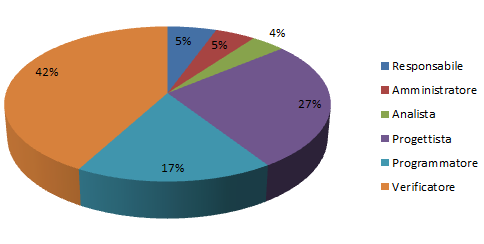
\includegraphics{torta_totale}
\caption{Torta ripartizione ruoli in tutto il periodo di svolgimento del Progetto MyTalk}\label{fig:oretotali}
\end{figure}
\clearpage

\subsubsection{Prospetto Economico}

Il Progetto nella sua realizzazione avrà un costo stimato calcolato nella tabella \ref{tab:costitotali} di seguito esposta, anche in questo caso il progetto impone un impegno economico coerente con i parametri imposti da capitolato.

\begin{table}[h!]
\centering
\begin{tabular}{|l|c|c|}
\hline
Ruolo& Ore& Costo\\
\hline
Responsabile & 40 & \EUR{1200} \\
Amministratore  & 33& \EUR{660}\\
Analista & 28& \EUR{700}\\
Progettista  & 193& \EUR{4246}\\
Programmatore & 124& \EUR{1860}\\
Verificatore & 303 & \EUR{4545}\\
\hline
Totale & 721 &\EUR{13.211,00}\\
\hline
\end{tabular}
\caption{costo e ore per ogni ruolo di progetto}\label{tab:costitotali}
\end{table}
\clearpage

\section{Consuntivo}
\subsection{Progettazione Architetturale}
Nell'attività di progettazione architetturale le differenze tempistiche ed economiche tra quanto preventivato e il consuntivo non sono state particolarmente rilevanti, se non a livello di distribuzione temporale e funzionali delle ore programmate.\
Le attività pianificate sono state correttamente avviate in data programmata, estendendo e correggendo i requisiti rilevati in attività di analisi per poi integrare il documento con le correzioni proposte dal committente sia a livello di requisiti che nella restante documentazione. Il termine dell'attività pianificata è stato al contrario anticipato di un giorno da parte del committente, portando la data ultima di consegna al 2013-01-30. Tale cambiamento non ha condizionato in modo rilevante il programma collettivo, in quanto le varie attività sono state svolte nei tempi previsti, consentendo inoltre l'inizio dell'attività di verifica anticipatamente su parti di documentazione già terminata.

\begin{figure}[h]
  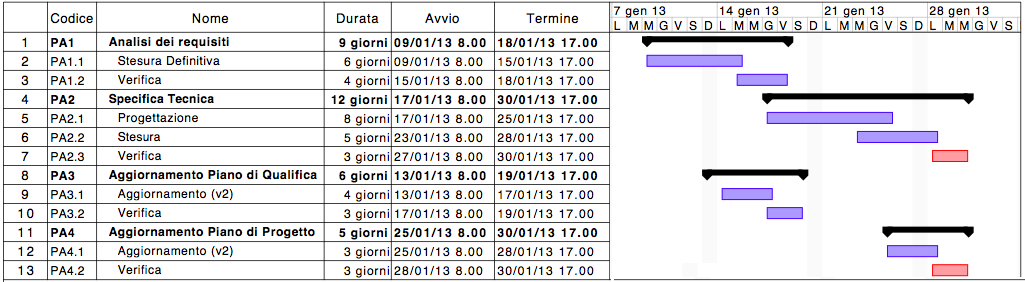
\includegraphics[width=\textwidth]{Consuntivo_Progettazione_Architetturale}
\caption{Gantt della Progettazione Architetturale}\label{fig:ganttprogconsuntivo}
\end{figure}

\begin{table}[h]
\centering
\begin{tabular}{|l|c|c|c|c|c|c|c|c|}
\hline
\multirow{2}{*}{Componente}& RE& AM& AN& PRO& PRO& PRG& VER& VER\\
                    &    &      &      &fase1          &fase2         &        &fase1	 &fase2\\ 
\hline
Diego Beraldin 	& & 5& \textcolor{green}{12}& & \textcolor{red}{18}& & &\\
Stefano Farronato & & & & 22& & & & \textcolor{green}{13}\\
Andrea Meneghinello & \textcolor{green}{6}& & & \textcolor{red}{15}& & & & 13\\
Andrea Rizzi & & 8& & & \textcolor{red}{19}& & \textcolor{green}{13}& \\
Marco Schivo & & & \textcolor{green}{13}& & 20& & & \\
Riccardo Tresoldi & \textcolor{green}{5}& & & 18& & & & 11\\
Elena Zecchinato & & & & & \textcolor{red}{18}& & \textcolor{green}{15}& \\
\hline
Totale & \textcolor{green}{11}& 13& \textcolor{green}{25}&\textcolor{red} {55}& \textcolor{red}{75}& & \textcolor{green}{28}& \textcolor{green}{37}\\
\hline
\end{tabular}
\caption{consuntivo orario dei ruoli nell'attività di Progettazione Architetturale}\label{tab:consruoliprog}
\end{table}

%Diego OK ore totali
%Stefano deve recuperare 3 ore totali
%Mene OK ore totali
%Rizzi OK ore totali
%Schivo deve recuperare 2 ore totali
%Tres deve recuperare 2 ore totali
%Elena deve recuperare 2 ore totali

Si può notare in particolare un discostamento quantificato attorno al 10\% di ore in eccesso per l'attività di progettazione architetturale e di circa il 25\% in difetto per l'attività di verifica. Nel primo caso ci sono state delle problematiche causate dall'inesperienza del team nel gestire tale attività, che hanno rallentato la fase preliminare della progettazione stessa, nel secondo è stato semplicemente sovrastimato il tempo necessario per la verifica dei documenti prodotti.

\begin{table}[H]
\centering
\begin{tabular}{|l|c c c c c c|c|}
\hline
Componente		& RE&   AM&   AN&  PRO& PRG& VER & TOTALE\\
\hline
Ore Preventivate	& 16&    13&   28&  115& 0&     81  & 253\\
Ore Effettive       	& 11 &   13&   25&  130& 0&     65 & 244\\
\hline
TOTALE			& \textcolor{green}{-5} &    0&    \textcolor{green}{-3}&    \textcolor{red}{+15}&0&    \textcolor{green}{-16} & \textcolor{green}{-9}\\
\hline
\end{tabular}
\caption{comparazione preventivo/consuntivo ore dell'attività di PA}\label{tab:consoreprog}
\end{table}

\begin{table}[H]
\centering
\begin{tabular}{|l|c c c c c c|c|}
\hline
Componente		& RE&   AM&   AN&  PRO& PRG& VER & TOTALE \\
\hline
Costo Preventivato  & \EUR{480}& \EUR{260}& \EUR{700}&\EUR{2530}& \EUR{0}& \EUR{1215} & \EUR{5185}\\
Costo Effettivo	       & \EUR{330}& \EUR{260}& \EUR{625}& \EUR{2860}&\EUR{0}& \EUR{975}& \EUR{5050}\\
\hline
TOTALE			& \textcolor{green}{\EUR{-50}} &    \EUR{0}&\textcolor{green}{\EUR{-75}}&   \textcolor{red}{\EUR{+330}}&\EUR{0}&   \textcolor{green}{\EUR{-240}} &\textcolor{green}{\EUR{-35}}\\
\hline
\end{tabular}
\caption{comparazione preventivo/consuntivo costi dell'attività di PA}\label{tab:concostisprog}
\end{table}

Dalle tabelle \ref{tab:consoreprog} e \ref{tab:concostisprog} riportate a pagina \vref{tab:concostisprog} si denota il risparmio di tempo e denaro stimato in 9 ore lavorative e per un totale di \EUR{35}. Tali risorse verranno reimpiegate nelle attività successive alla Progettazione Architetturale qualora se ne manifestasse la necessità.

\subsubsection{Preventivo a finire -- PA}

In base ai dati e alle esperienze raccolte durante l'attività di progettazione architetturale, il team ha preventivato per la prossima attività di progettazione di dettaglio e codifica che le ore destinate alla progettazione probabilmente subiranno una lieve contrazione, per dar spazio ad eventuali verifiche più accurate integrando eventualmente le risorse non utilizzate nell'attività di progettazione architetturale.
Purtroppo al momento attuale non ci sono ulteriori basi per valutare ulteriori modifiche alla pianificazione relativa alla progettazione di dettaglio e codifica, pertanto verrà seguita la pianificazione redatta senza ulteriori modifiche sostanziali.
Concludiamo la sezione aggiornando il costo e le ore totali destinate al progetto che il committente ha accettato in revisione dei requisiti.

\begin{table}[h!]
\centering
\begin{tabular}{|l|c|c|}
\hline
Tipologia&Preventivo iniziale& Prevetivo a finire \\
\hline
Orario & 721& \textcolor{green}{712} \\
Economico & \EUR{13.211,00} &\textcolor{green}{\EUR{13.176,00}}\\
\hline
\end{tabular}
\caption{costo e ore preventivo a finire}\label{tab:conspa}
\end{table}

\subsection{Progettazione di Dettaglio e Codifica}
\subsubsection{Preventivo a finire - PDC}

\clearpage


\clearpage
\section{Analisi dei rischi di progetto}

In questa sezione vengono analizzati in modo mirato e approfondito i rischi che si sono individuati come possibili durante lo svolgimento del progetto. L'individuazione e la strategia di mitigazione di tali rischi è fondamentale per la pianificazione delle attività e la loro corretta esecuzione, infatti solo tramite un approccio di gestione ai fattori di rischio è possibile tutelarsi dalla loro eventuale insorgenza e mitigarne gli effetti.

Data la scarsa esperienza del team su tali tematiche, il gruppo si è affidato a delle sessioni di \underline{\inglese{brainstorming}} collettive cercando di focalizzare i vari punti critici.

Per rendere efficace l'analisi di ogni rischio si è deciso di quantificarlo mediante un apposita scala di valutazione sia dal punto di vista della probabilità che il rischio si manifesti (livello), sia il suo grado di incidenza sul progetto stesso (impatto):

\begin{table}[h!]
\centering
\begin{tabular}{|l|c|}
\hline
Probabilità& Descrizione\\
\hline
ALTA & probabilità elevata che si verifichi\\
MEDIA & probabilità equivalente nel verificarsi o meno\\
BASSA & probabilità bassa che si verifichi\\
\hline
\end{tabular}
\caption{Probabilità e Descrizione probabilità di un rischio}\label{tab:livellorischi}
\end{table}
\begin{table}[h!]
\centering
\begin{tabular}{|c|c|}
\hline
Scala& Descrizione  \\
\hline
5 & conseguenze molto gravi\\
4 & conseguenze gravi\\
3 & conseguenze medio-gravi\\
2 & conseguenze minimali\\
1 & nessuna/lievi conseguenze\\
\hline
\end{tabular}
\caption{Scala e descrizione delle conseguenze di un rischio}\label{tab:impattorischi}
\end{table}

\subsection{Problemi personali}

\begin{description}
	\item{\scshape\bfseries Analisi:} durante la realizzazione del progetto è probabile che alcuni membri del team siano soggetti a problemi fisiologici e/o sovvengano impegni personali improrogabili che porterebbero ad una sicura modifica della pianificazione del lavoro collettivo. L'impatto di tale rischio è variabile in base al soggetto mancante, in quanto può essere assegnato ad un'attività (o ruolo) più o meno importante all'interno del progetto.
	\item{\scshape\bfseries Probabilità:} ALTA
	\item{\scshape\bfseries Impatto:} variabile
	\item{\scshape\bfseries Strategia di Gestione:}per mitigare gli effetti di tali fenomeni è ragionevole prima di tutto pianificare i tempi di lavoro personali in modo da lasciare un lasco temporale tra un attività e l'altra.
	
Così facendo la gestione temporale (compresa di eventuali imprevisti) risulta meno incline a modifiche e/o cambiamenti dei ruoli assegnati ad ogni membro. Ovviamente anche adottando tali accorgimenti si potrà generare la situazione in cui un componente risulti impossibilitato a svolgere il proprio compito, in tal caso è buona norma che tutti i membri siano ben preparati (conoscenza del dominio e delle metodologie di lavoro) nel caso sia necessaria la sostituzione momentanea del soggetto.

	\item{\scshape\bfseries Riscontro effettivo:} nel periodo trascorso sino alla la progettazione di dettaglio e codifica i componenti del team hanno lavorato con costanza e segnalato con discreto anticipo eventuali assenze giustificate. Tali premesse hanno consentito una corretta esecuzione dei compiti fin'ora assegnati senza particolari difficoltà, pertanto possiamo affermare grazie ad una strategia di gestione efficace e un'alta disponibilità da parte dei membri tale rischio risulta attualmente mitigato correttamente.
	
Viene inoltre sottolineata (anche se non specificata nel rischio in questione) una coesione produttiva da parte del gruppo, consentendo una collaborazione senza particolari attriti tra i componenti del gruppo stesso. Non si sono pertanto verificati pertanto problemi interpersonali che avrebbero potenzialmente minato la stabilità e la serenità dell'ambiente lavorativo. 
\end{description}

\subsection{Variazione nei Requisiti}

\begin{description}
	\item{\scshape\bfseries Analisi:} il bando di capitolato non prevede modifiche per i requisiti obbligatori, i requisiti opzionali al contrario possono subire variazioni in corso d'opera. Tale situazione implica il rischio che le risorse assegnate durante l'attività pianificazione risultino insufficienti al soddisfacimento di tali requisiti.
	\item{\scshape\bfseries Probabilità:} MEDIA
	\item{\scshape\bfseries Impatto:} 3
	\item{\scshape\bfseries Strategia di Gestione:}risulta necessaria una doverosa e immediata ridistribuzione delle risorse cercando di mantenere limitato l'impatto sulla pianificazione originale.
	\item{\scshape\bfseries Riscontro effettivo:} i requisiti espressi non sono mutati in modo significavo durante le attività fin'ora svolte, le modifiche imposte in RR e RP non hanno portato variazioni così rilevanti da richiedere ulteriori sforzi non preventivati. Possiamo pertanto ritenere il rischio controllato nelle attività fin'ora svolte.
\end{description}

\subsection{Scarse conoscenze tecnologiche}
\begin{description}
	\item{\scshape\bfseries Analisi:} per ovvie ragioni di inesperienza da parte di tutto il team buona parte delle competenze tecnologiche richieste per la realizzazione del progetto risultano sconosciute.
	\item{\scshape\bfseries Probabilità:} ALTO
	\item{\scshape\bfseries Impatto:} 3
	\item{\scshape\bfseries Strategia di Gestione:} le lacune saranno colmate tramite la personale consultazione della documentazione specifica che ogni tecnologia fornisce. Inoltre periodicamente, su base volontaria, specifici componenti si assumeranno l'incarico di redigere brevi relazioni di facile e mirata comprensione sulle tecnologie prese in esame.
	\item{\scshape\bfseries Riscontro effettivo:} l'inesperienza dei componenti del team sulle tecnologie specifiche utilizzate fino all'attività di progettazione di dettaglio e codifica hanno imposto ulteriori sforzi a quelli preventivati. Tale rischio, correttamente preventivato con probabilità alta si è manifestato e si è cercato di gestirlo come redatto precedentemente con risultati generali accettabili. 
\end{description}

\subsection{Variabili Tecnologiche}

\begin{description}
	\item{\scshape\bfseries Analisi:} tra le tecnologie di implementazione sono presenti le librerie \underline{WebRTC} e \underline{HTML5}. Ad oggi tali progetti non sono ancora stati promossi a standard ma risultano in una fase di sviluppo costante. Seppur HTML5 risulti ormai discretamente stabile nella sua implementazione, WebRTC al contrario si presta a periodiche modifiche strutturali, l'ultima delle quali è avvenuta il 15 novembre 2012 (a tempo di redazione del documento).
	\item{\scshape\bfseries Probabilità:} MEDIA
	\item{\scshape\bfseries Impatto:} 2
	\item{\scshape\bfseries Strategia di Gestione:} questa condizione ci chiede di prestare massima attenzione durante l'attività di progettazione, al fine di rendere il prodotto ultimo più flessibile possibile. Il proponente in ogni caso è disposto ad accettare una prodotto funzionante con una versione più datata rispetto a quella che verrà ad essere ufficiale in data di accettazione.
	\item{\scshape\bfseries Riscontro effettivo:} nonostante WebRTC subisca aggiornamenti minori regolarmente, tali cambiamenti non si sono rivelati particolarmente critici al punto di minare la fattibilità del progetto analizzata nelle fasi iniziali. Possiamo pertanto affermare che tale rischio risulta non ancora verificato.
\end{description}

\subsection{Errata stima di Risorse}
\begin{description}
	\item{\scshape\bfseries Analisi:} l'errata pianificazione del lavoro in particolare nella distribuzione delle ore svolte da ogni ruolo (sia in eccesso che in difetto) fanno parte dell'ovvia inesperienza del team nella gestione di tali tematiche. Tali errori di stime possono portare ad uno sbilanciamento dei costi (sia in eccesso che in difetto) che andrà ad incidere nel bilancio finale.
	\item{\scshape\bfseries Probabilità:} MEDIA
	\item{\scshape\bfseries Impatto:} 3
	\item{\scshape\bfseries Strategia di Gestione:} risulterà indispensabile da parte dei componenti del team la massima flessibilità nel cambiamento dei ruoli, sarà compito del responsabile ridirigere le risorse nel modo più adeguato e prestando particolare attenzione ad eventuali conflitti di ruoli.
	\item{\scshape\bfseries Riscontro effettivo:} sono state effettuate delle modifiche più o meno significative alle ore assegnate ai componenti nell'esecuzione delle varie attività, fortunatamente al contrario non sono state necessarie riassegnazioni di risorse precedentemente destinate ad altri compiti; il rischio risulta pertanto attualmente gestito: ogni componente ha finora svolto gli incarichi pre assegnati.
\end{description}

\subsection{Problemi Software/Hardware}
\begin{description}
	\item{\scshape\bfseries Analisi:} sono ovviamente probabili eventuali disguidi di natura tecnica, sia di natura hardware (guasti/problemi tecnici generici delle macchine) che software. E' altresì probabile che software diversi all'interno dello stesso sistema operativo risultino di difficile integrazione, inoltre il progetto stesso che per sua natura si presta ad essere utilizzato su vari \underline{browser} (oltre a \underline{Chrome}, di default) potrebbero presentare problemi di natura funzionale. Infine si sottolinea che i componenti del team dispongono di sistemi basati su piattaforme differenti che potrebbero far insorgere incompatibilità.
	\item{\scshape\bfseries Probabilità:} MEDIA
	\item{\scshape\bfseries Impatto:} 4
	\item{\scshape\bfseries Strategia di Gestione:} questo tipo di problematiche andranno affrontate caso per caso, è stata comunque preventivata un esigua parte di tempo per gestire tali tematiche nella pianificazione del lavoro.
	\item{\scshape\bfseries Riscontro effettivo:} la pianificazione temporale dedicata alla configurazione delle risorse software e l'auto apprendimento dei vari componenti del team sono stati sufficienti per prendere confidenza con i programmi e testarne la compatibilità e integrazione con le piattaforme utilizzate.
A livello hardware non si sono riscontrati finora problemi negli strumenti in dotazione del gruppo. Il rischio pertanto risulta attualmente gestito correttamente per la parte software, mentre non pervenuto a livello hardware.
\end{description}

% TODO: 
% da aggiungere capitolo note a consuntivo con sezione "dalla RR alla RP" in cui descriviamo quanto accaduto fra le due milestone

\end{document}
